\documentclass[12pt]{article}
\usepackage{graphicx}
\usepackage{geometry}
\geometry{margin=82pt}

\begin{document}

\section*{Backpropagation Neural Network}
\begin{figure}[h!]
\center
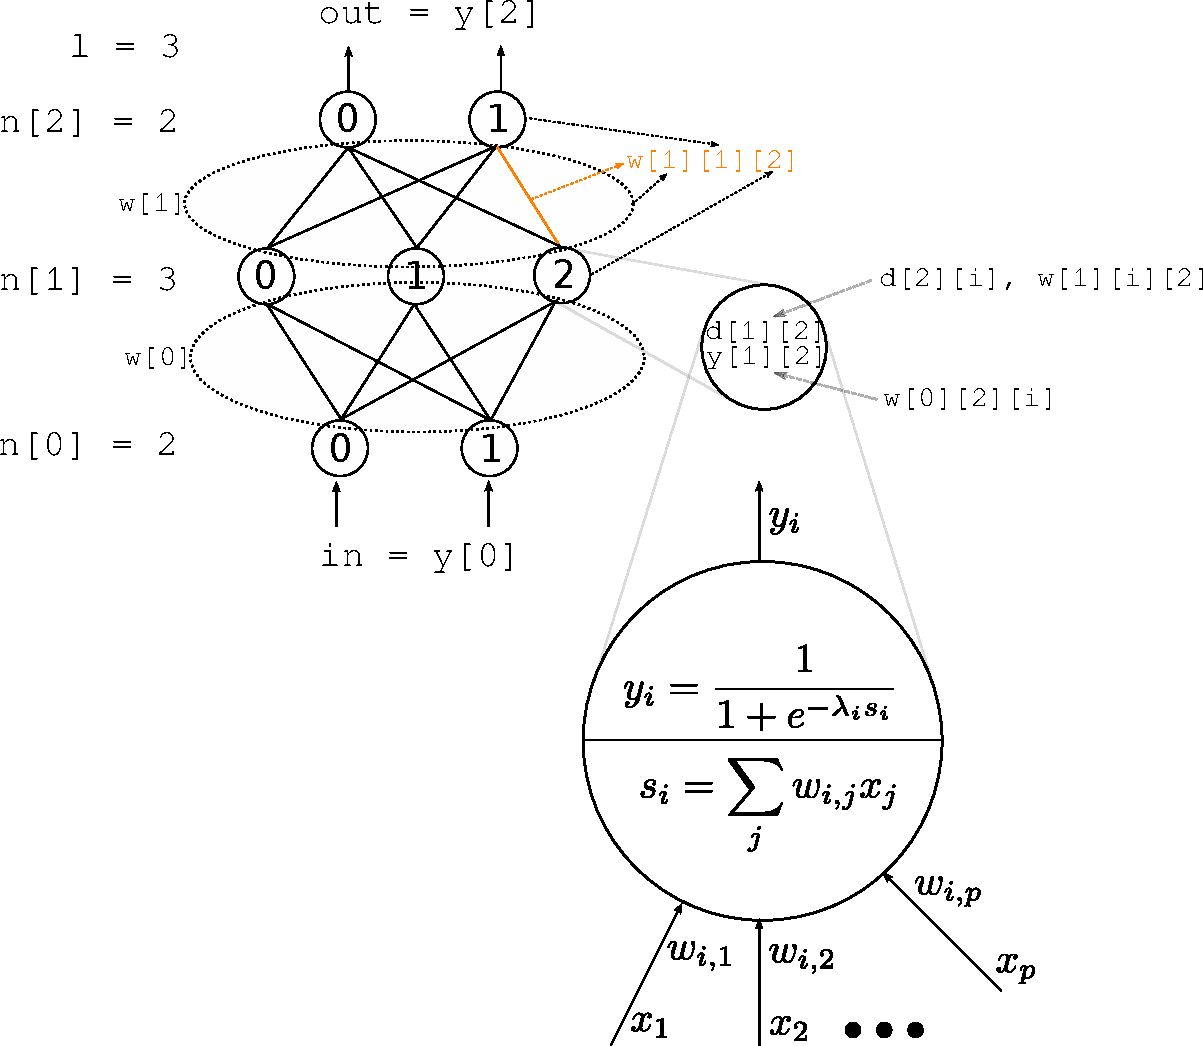
\includegraphics[width=0.9\textwidth]{drawing.pdf}
\caption{Neural Network Model}
\label{fig:1}
\end{figure}

The potential of neuron $i$ in a layer $k$ is defined as the weighted sum of all inputs to the neuron, i.e.
\begin{equation}
\label{eq:1}
s_{k,i} = \sum_{j} w_{k-1,i,j}\:  y_{k-1,j} \, ,
\end{equation}
where $w_{k-1,i,j}$ is the weight between a neuron $i$ from the $k$-th layer and a neuron $j$ from the $(k-1)$-st layer, $y_{k-1,j}$ is the input to the neuron $i$ (output of the neurons from the previous layer).
If this potential is higher than a threshold value, the neuron is excited to the value $1$, otherwise it is inhibited to the value $0$.
The value of the excitation depends on an activation function.
For this purpose, we use the sigmoid function.
Let $y_{k,i}$ be the output of the neuron $i$ in the layer $k$. 
The output (the excitation value) is defined as
\begin{equation}
\label{eq:2}
y_{k,i} = \frac{1}{1+e^{-\lambda s_{k,i}}} \, .
\end{equation}

The error of the network is given by the values of $y$ in the output layer comparing to the expected values.
Let us assume that we have a neural network with $3$ layers - input layer, one hidden layer, and output layer (as shown in Fig.~\ref{fig:1}).
The output layer contains two neurons, therefore, the expected output on a given input is represented by two values.
Let us now assume that we want to classify the objects into two classes (square and rectangle) using our features $F1$, $F2$.
Let the output of first neuron in the output layer $y_{2,0}$ be the probability that the features represent the square object.
Similarly, let $y_{2,1}$ be the probability that the features represent the rectangular object.
For the square, the expected values are $y_{2,0} = 1$, $y_{2,1}=0$.
For the rectangle, it is $y_{2,0} = 0$, $y_{2,1}=1$.
The error of the network is given by the difference between the expected and the real output.
Let $t_i$ be the expected output of the neuron $i$.
Then the error of the network is defined as
\begin{equation}
\label{eq:3}
E = \frac{1}{2} \sum_{i}(t_i - y_{2,i})^2 \, .
\end{equation}
The goal is to minimize this error.
This minimization is done via changing the weights between the neurons.
For this purpose, the backpropagation is used, which is an algorithm minimizing the error by a gradient method.
The weights are iteratively changing until the error of the network is lower than a chosen threshold (or until a number of iterations is reached).
The computation of the new weights is different for the output layer and for the hidden layers (the derivation of the formulas is in [1]).
For the output layer, the error of the neuron is computed as
\begin{equation}
\label{eq:4}
d_{k,i} = (t_{i} - y_{k,i}) \: \lambda \: y_{k,i} \: (1-y_{k,i}) \, .
\end{equation}
For the hidden layer, the error of a neuron $i$ in a layer $k$ is influenced by the errors of the neurons $j$ from the layer $(k+1)$.
Therefore, the error is computed as
\begin{equation}
\label{eq:5}
d_{k,i} = \Big( \sum_j d_{k+1,j} \: w_{k,j,i} \Big) \lambda \: y_{k,i} \: (1-y_{k,i}) \, .
\end{equation}
The weights in the network are then changed by 
\begin{equation}
\label{eq:6}
\Delta w_{k,i,j} = \eta \: d_{k+1,i} \: y_{k,i} \, .
\end{equation}
\subsubsection*{Your task}
The neural network is prepared in the template files (\texttt{backprop.cpp} and \texttt{backprop.h}). All the variables are prepared and are called in the same way as in this text (and also as in Fig.~\ref{fig:1}).
Your task is to create the methods \texttt{feedforward} and \texttt{backpropagation}. 
The \texttt{feedforward} method takes the input vector (\texttt{y[0]}), passes it through the network and sets the output (\texttt{y[2]}).
You will use Eqs.~(\ref{eq:1}, \ref{eq:2}).
The \texttt{backpropagation} computes the error of the network using Eq.~(\ref{eq:3}), and sets the new weights between the neurons using Eqs.~(\ref{eq:4}, \ref{eq:5}, \ref{eq:6}).
Train your neural network to classify the objects (square, rectangle, star, circle) using the features $F1$-$F3$ obtained from the training image.
Afterwards, test your neural network to classify the objects in the testing image.


\end{document}
